\documentclass[mathserif, aspectratio=169]{beamer}

\usepackage{movie15}
\usepackage{psfrag,graphicx}
\usepackage{amsmath}
\usepackage[absolute,overlay]{textpos}
\usepackage{tikz}
\graphicspath{{figs/}}

\usetheme{Boadilla}
\makeatother
\setbeamertemplate{footline}[frame number]

\usepackage{graphicx}
\usepackage{caption}
\usepackage{subcaption}
\captionsetup{compatibility=false}
\usepackage{amsmath} 
\usepackage{amssymb} 
\usepackage{amsthm}  
\usepackage{bm}
\usepackage{lipsum}
\usepackage[linesnumbered, ruled]{algorithm2e}
\usepackage{color}
\newtheorem{assumption}{Assumptions}
\newtheorem{prop}{Proposition}
\newtheorem{defn}{Definition}
\newtheorem{thm}{Theorem}
\newtheorem{lem}{Lemma}
\newtheorem{cor}{Corollary}
\newtheorem{sol}{Decentralized Solution}
\newtheorem{thresh}{$\epsilon$-thresholding}
\definecolor{light-gray}{gray}{0.8}
\usepackage{textcomp}

\newcommand{\backupbegin}{
   \newcounter{finalframe}
   \setcounter{finalframe}{\value{framenumber}}
}
\newcommand{\backupend}{
   \setcounter{framenumber}{\value{finalframe}}
}
\newcommand{\norm}[1]{\left\lVert #1 \right\rVert}

\makeatletter
\setbeamertemplate{navigation symbols}{}



\title[Lecture 23] % (optional, use only with long paper titles)
{Data, Environment and Society: \\{Lecture 23: Boosting, Bagging and Random Forests}}



\author[ER190C: Data, Environment and Society] 
{Instructor: Duncan Callaway\\
GSI: Seigi Karasaki} 

%\logo{
%\includegraphics[width=1.5cm,height=1.5cm,keepaspectratio]{uvic_logo_h.jpg}
%}
\vspace{-20mm}
\institute[UC Berkeley] % (optional, but mostly needed)
 {\small{ \bf November 8, 2018}}


\date[November 8, 2018]


\begin{document}

\frame{
  \titlepage
}

\begin{frame}{Announcement}

\begin{itemize}
\item Projects!
\begin{itemize}
\item Data identified and ``resource allocation'' question by 11/19 lab.
\item First pass on running a prediction model by 11/26 lab.
\item Lab notebook due Dec 11, 6pm (when the final exam would have ended).
\item Come to office hours, or schedule time with us, to discuss your ideas!
\end{itemize}
\item Next week
\begin{itemize}
\item We'll begin talking about support vector machines Tuesday
\item Thursday, guest lectures from Grace Wu and Diego Ponce de Leon Barido.
\begin{itemize}
\item Support vector machines played a prominent role in Grace's PhD work on impact of dams on deforestation!
\item Diego focuses on energy data analytics and sharing in Latin America
\end{itemize}
\end{itemize}
\item Remainder of semester
\begin{itemize}
\item Finish support vector machines on 11/20
\item Quick intro to neural networks on 11/27
\item Duncan traveling 11/29...
\end{itemize}
\end{itemize}


\end{frame}

\begin{frame}{Today's lecture setup}

Thus far we've talked about regression trees and classification trees.
\begin{itemize}
\item We build multiple trees in the cross validation process
\item But then build a single tree with all folds.
\end{itemize}

\only<1>{
\begin{figure}
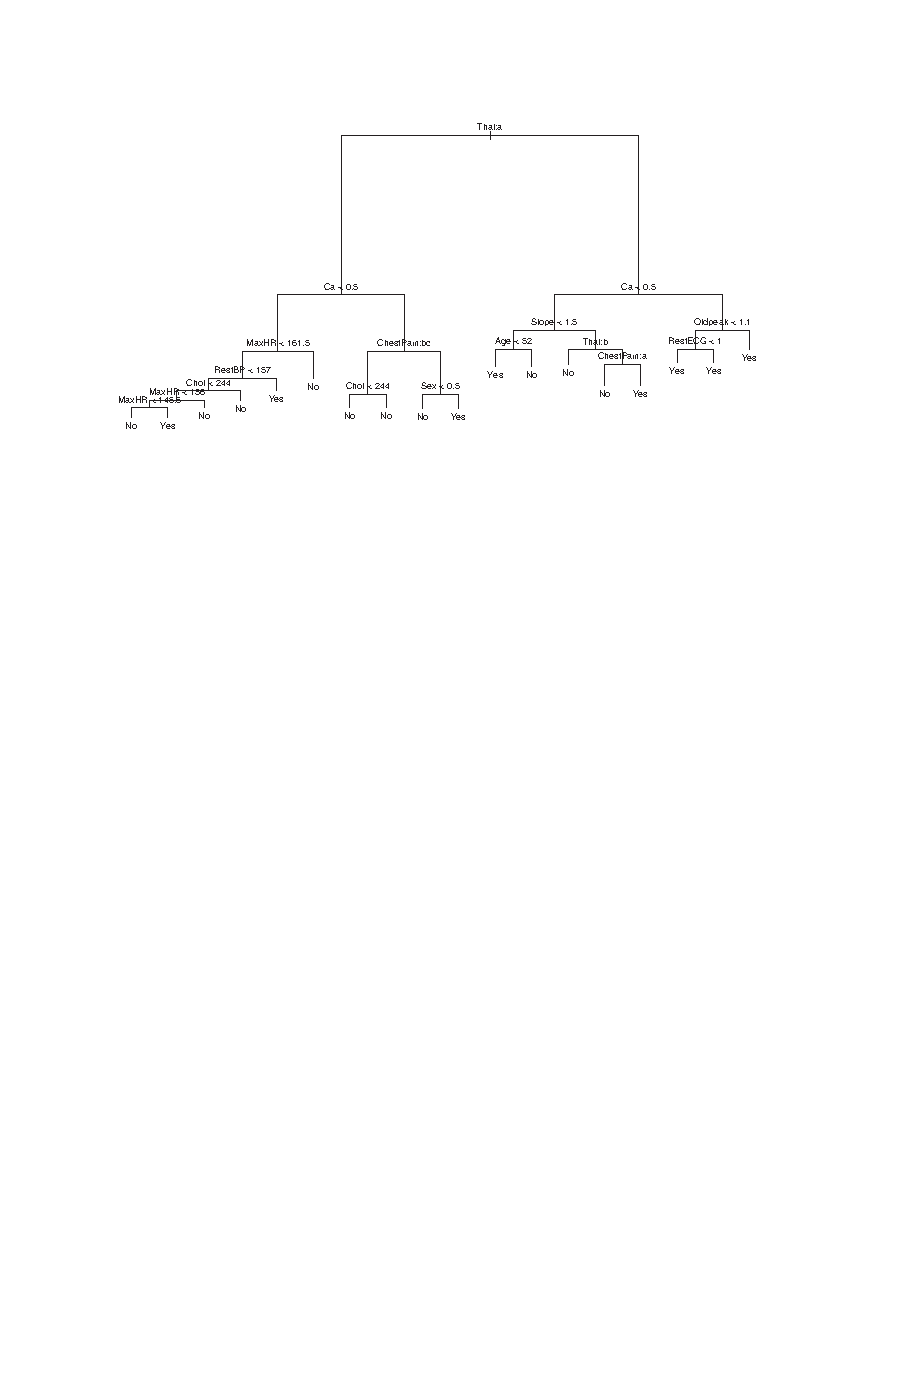
\includegraphics[scale=0.9]{heart_tree}
\caption*{From ISLR: Heart disease classification tree}
\end{figure}}

\only<2>{
\begin{figure}
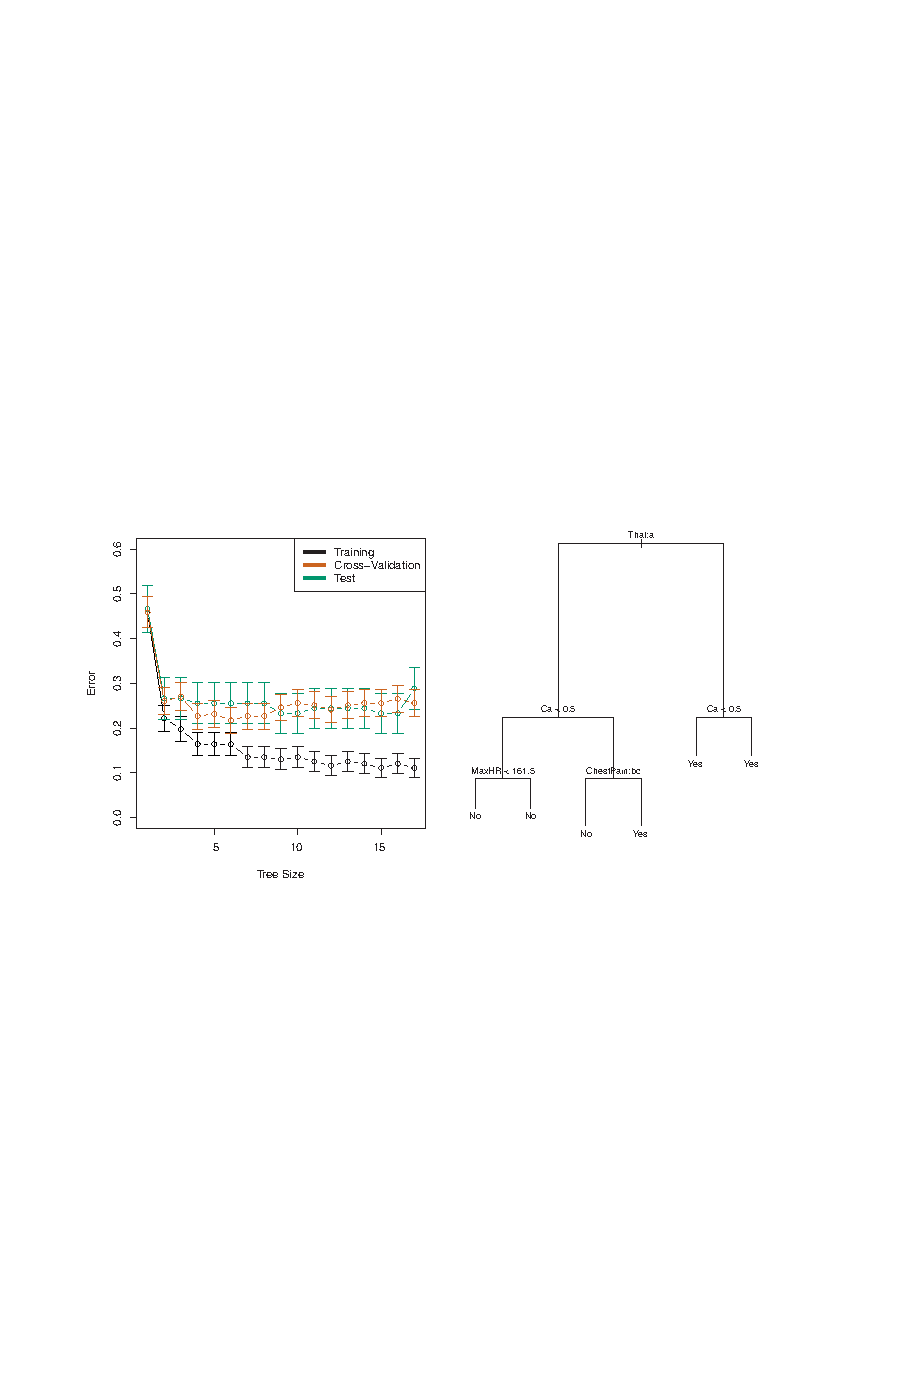
\includegraphics[scale=0.9]{heart_tree_pruned}
\caption*{From ISLR: Heart disease classification tree}
\end{figure}}


\uncover<3->{
As we've discussed:
\begin{itemize}
\item Recursive binary splitting quickly narrows the set of candidate trees 
\item The ``best'' tree might be one with a different first split than the ``greedy optimal'' one.
\end{itemize}

Trees built using the approaches we've learned so far tend to have \textit{high variance.}  \\~\\

\textbf{Why?}}
\uncover<4->{\begin{itemize}
\item Split the data randomly into two data sets
\item Each one could yield very different trees, depending on the nature of the random split.  \\~\\
\end{itemize}

Today we'll talk about tools to bring the variance down.}

\end{frame}

\begin{frame}{How much does this cow weigh?}

\begin{figure}
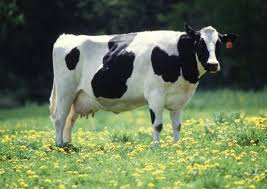
\includegraphics[height=0.75\textheight]{cow.jpg}
\caption*{\uncover<2->{According to James Surowiecki's book, \textit{The Wisdom of Crowds}, in 1906 Frances Galton averaged all of a crowd's guesses for a heffer and they were only 1\% off.}}
\end{figure}
\end{frame}

\begin{frame}{Another anecdote}

The Netflix Prize: Use historical viewing data to predict what movies customers will like.  \\~\\

\pause
The winners were like the crowd at that 1906 county fair: they were a coalition of three separate competitors from the prior year.  They averaged their models, won, and split the winnings three ways.\\~\\

\begin{figure}

\includegraphics[width=\textwidth]{netflix}
\caption*{}
\end{figure}

\end{frame}
\begin{frame}{Overview of how ``the power of crowds'' works for regression trees.}

Step 1: Accept that interpretability is a casualty for what you're about to do\\~\\
\pause
Step 2: Build many different trees from the data you're given\\~\\
\pause
Step 3: \textit{Average }the predictions from many different trees.\\~\\
\pause
Interpretability is lost: now there are many trees with splits in different locations on different predictors.  \\~\\

But if it's done right: You'll get better \textit{predictions} because you'll reduce variance\\~\\

\textbf{Different methods differ in step two}: how do you manipulate the tree building process so that you get different trees built from the same data?

\end{frame}

\begin{frame}{Three ways to build many trees from the same data}

\begin{itemize}
\item \textbf{Bagging} (Bootstrap aggregation): Build many trees from random samples of the data
\item \textbf{Random forests}: Build many trees from bootstrapped samples, but each binary split is chosen from a random subset of predictors
\item \textbf{Boosting}: choose new trees to minimize the residual of an existing aggregation of trees.
\end{itemize}
\end{frame}

\begin{frame}{}

\begin{center}
\LARGE Bagging = Bootstrap aggregating
\end{center}

\begin{columns}
\column{0.3\textwidth}
Leo Breiman retired from UC Berkeley Statistics in 1993 and published the first paper on bagging in 1994.  \\~\\

\column{0.5\textwidth}
\begin{figure}
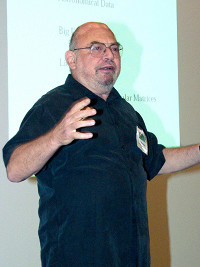
\includegraphics[width=0.6\textwidth]{Leo_Breiman}
\caption*{}
\end{figure}
\end{columns}
\end{frame}

\begin{frame}{Reminder: Bootstrapping}

Suppose you want to compute the standard error for a metric, but you can't get there with conventional statistics:

\begin{figure}
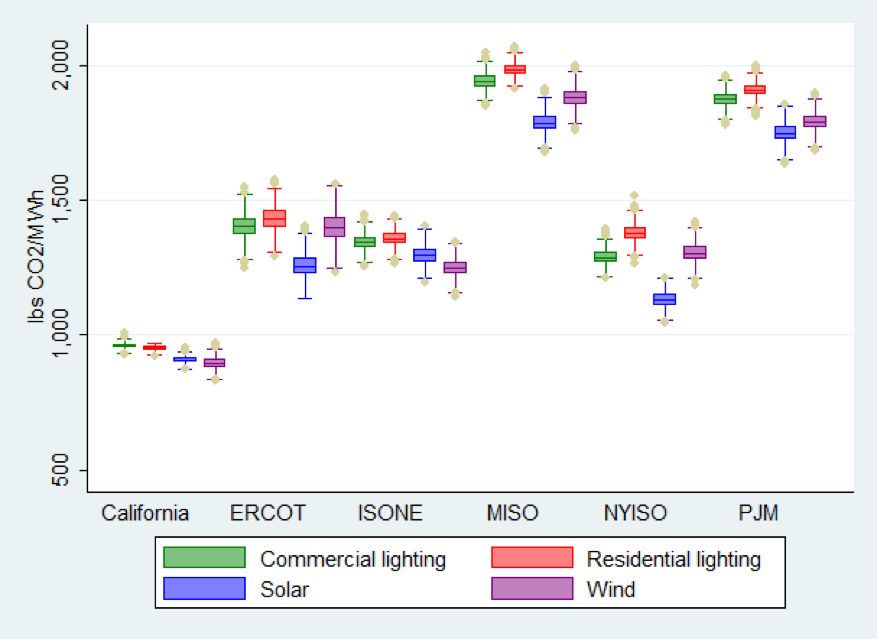
\includegraphics[height=0.7\textheight]{MEDR}
\caption*{\tiny (Callaway, Fowlie, McCormick 2017)}
\end{figure}
\end{frame}

\begin{frame}{Reminder: Bootstrapping, Part 2}

\begin{columns}
\column{0.5\textwidth}

\begin{itemize}
\item \textit{First key idea}: create a new sample of $N$ observations from your original ($N$ observation) sample by sampling with replacement.
\item Repeat this $B$ times
\item Record the metrics you care about each time you build a new model from a new bootstrap
\item The average parameter estimate will equal the true parameter
\item \textit{Second key idea}:  the standard error of the parameter estimates from the population of boostrapped estimates will be roughly the true standard error.
\end{itemize}
\column{0.5\textwidth}
\begin{figure}
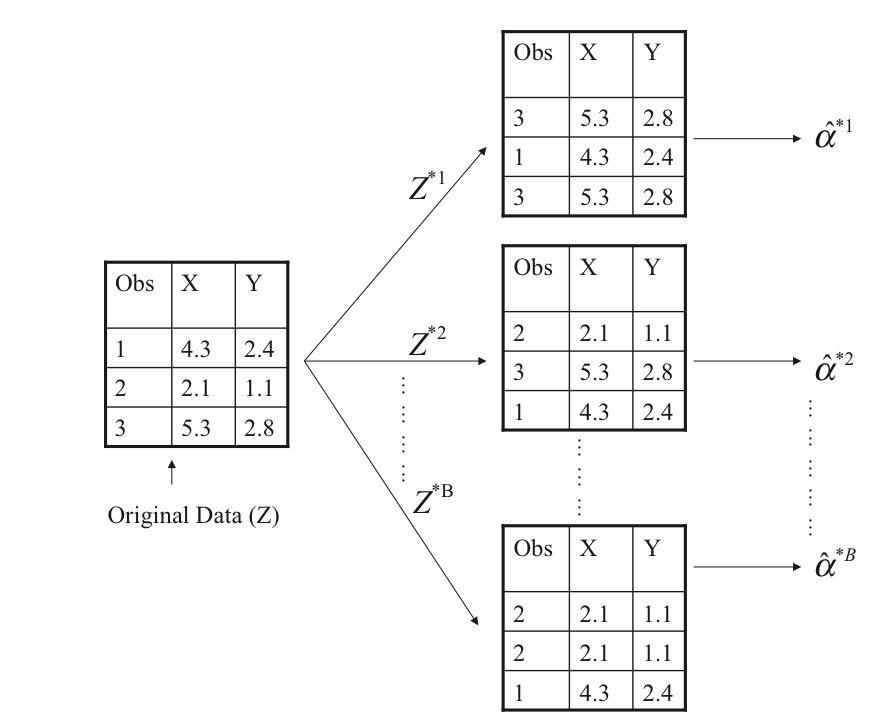
\includegraphics[width=\textwidth]{bootstrap}
\caption*{}
\end{figure}
\end{columns}
\end{frame}

\begin{frame}{Examples of things you might bootstrap}
\begin{itemize}
 \item A prediction of PM2.5 concentration at a new location
 \item An estimate for how many CO2 emissions were displaced by a low-carbon technology
 \item An estimate of the number of people that died due to ozone for a given set of predictors
 \end{itemize} 
\end{frame}

\begin{frame}{Moving on to \textbf{B}ootstap \textbf{AGG}regat\textbf{ING} = Bagging}

It's very simple: 

\begin{align*}
\hat{f}_\text{bag}(x) = \frac{1}{B}\sum_{b=1}^B \hat{f}^{*b}(x)
\end{align*}

where $\hat{f}^{*b}(x)$ is the regression tree estimate from the $b^\text{th}$ bootstrapped data set.\\~\\

Each individual tree has high variance but low bias.  But averaging deals with the variance.\\~\\

\pause

Important: because we deal with variance by averaging, there is no more need for cost-complexity pruning or tuning of the $\alpha$ parameter. \\~\\

Consequence: Grow the trees deep!

\end{frame}

\begin{frame}{Further details}

\begin{columns}

\column{0.5\textwidth}
Data set and model: predict patients' heart disease condition (yes or no) based on many observations.

\vspace{5mm}

\textbf{How many bootstraps?}  As with conventional boostrapping, keep adding boostraps until the estimate converges.  

\column{0.5\textwidth}
\vspace*{-10mm}
\begin{figure}
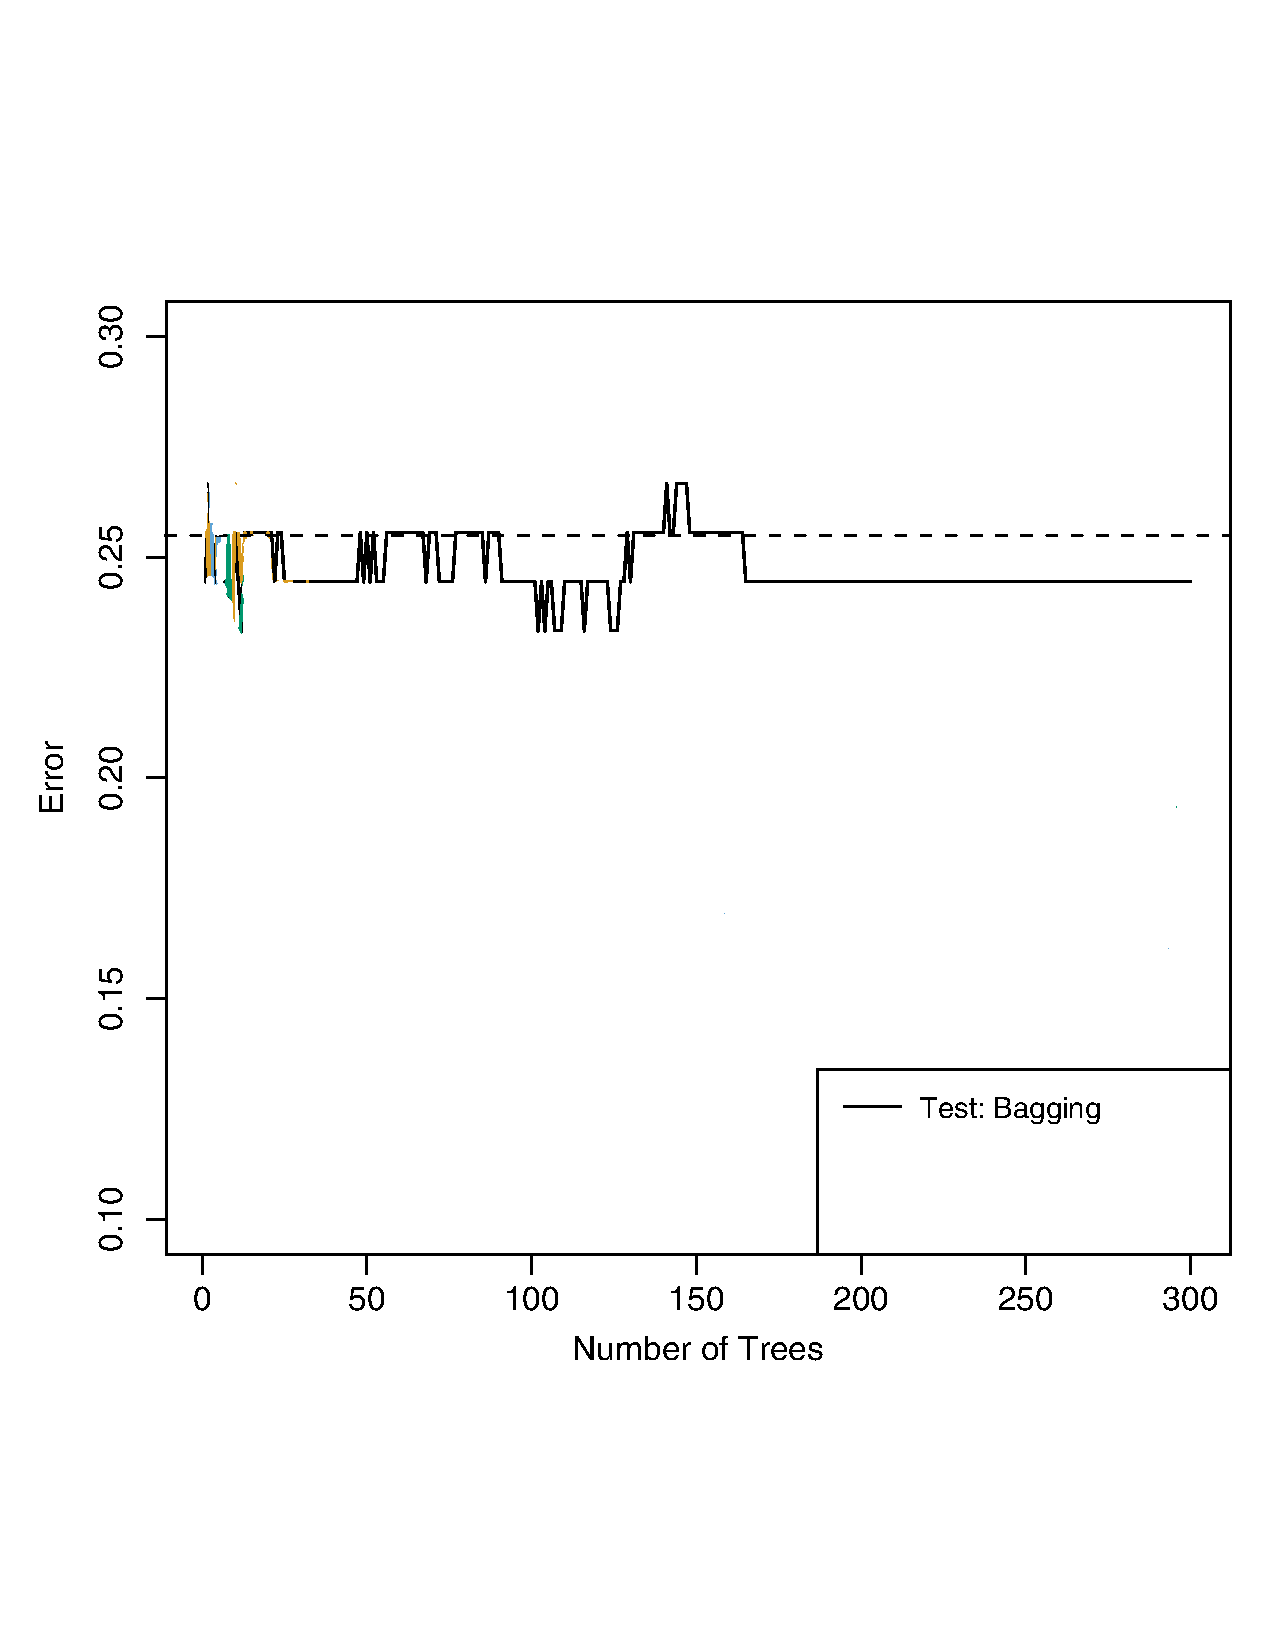
\includegraphics[width=0.9\textwidth]{islr88_only_bag.pdf}
\caption*{\footnotesize Bagged model (black) vs single regression tree (dashed).  Only look at \textit{Test: Bagging} for now.}
\end{figure}
\end{columns}
\pause

\textbf{Classification with Bagging}: just take the ``majority vote'' from all the trees you build.

\end{frame}

\begin{frame}{``Out of bag''? The terminology keeps getting better!}

When you bootstrap with replacement, a certain number of observations don't get chosen for inclusion in the sample.  
\begin{itemize}
\item Folks call those the Out Of Bag observations.
\item On average an observation will be left out of about 1/3rd of the bootstrap samples\\~\\
\end{itemize}

\pause\pause
OOB error for an observation: difference between an observation and its prediction using the average of the models built with the observation out-of-bag.  This can be MSE or classification error.\\~\\

OOB error for the model is the mean OOB across all observations.  

\end{frame}

\begin{frame}{Why OOB is useful}

\begin{itemize}
\item Valid estimate of the test error for the bagged model, 
\begin{itemize}
\item The response for each observation is predicted using only the trees that were not fit using that observation. \\~\\
\end{itemize}
\item With $B$ sufficiently large, OOB error is virtually equivalent to leave-one-out cross-validation error
\begin{itemize}
\item This means you can get an estimate of LOOCV error without actually having to do LOOCV.
\item Unlike many other nonlinear estimators, random forests can be fit in one sequence, with cross-validation being performed along the way
\end{itemize}
\end{itemize}
\end{frame}

\begin{frame}{Let's look at OOB error}

\begin{figure}
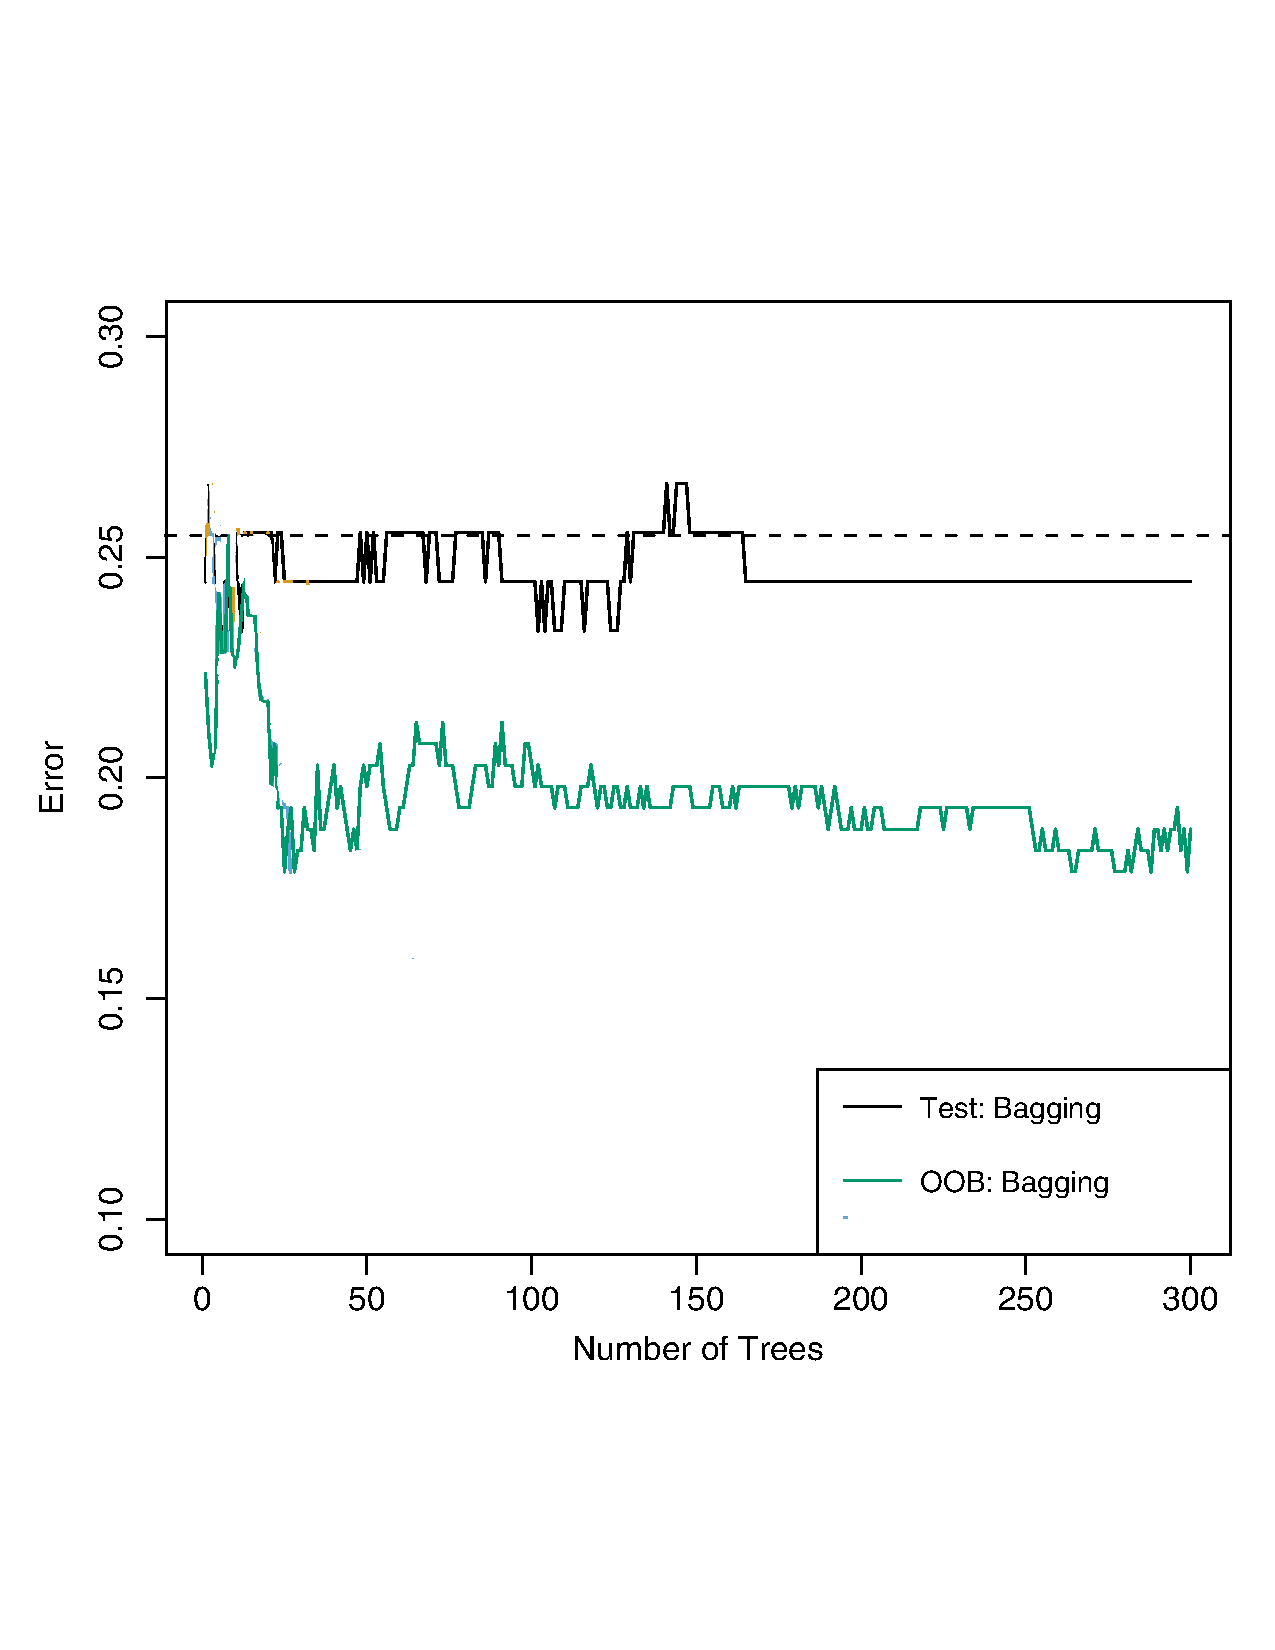
\includegraphics[height=0.85\textheight]{islr88_BagAndOOB.pdf}
\caption*{}
\end{figure}
\end{frame}

\begin{frame}{Interpretation is not entirely lost: Variable importance measures.}

Basic idea: 
\begin{enumerate}
\item For each predictor indexed by $j$, initialize a variable $\rho_j =0$
\item Then as you grow the trees, every time you split on predictor $j$ add the improvement in RSS for the split to $\rho_j$.  
\begin{itemize}
\item (As you move to a new tree you can keep adding to the same $\rho_j$s, no need to start anew.)
\end{itemize}
\item When you're done growing trees, normalize all $\rho$ to $\frac{\rho_j}{\max{\rho_j}}*100$
\end{enumerate}

\end{frame}

\begin{frame}{Example Variable Importance Measures - Heart data}

\begin{figure}
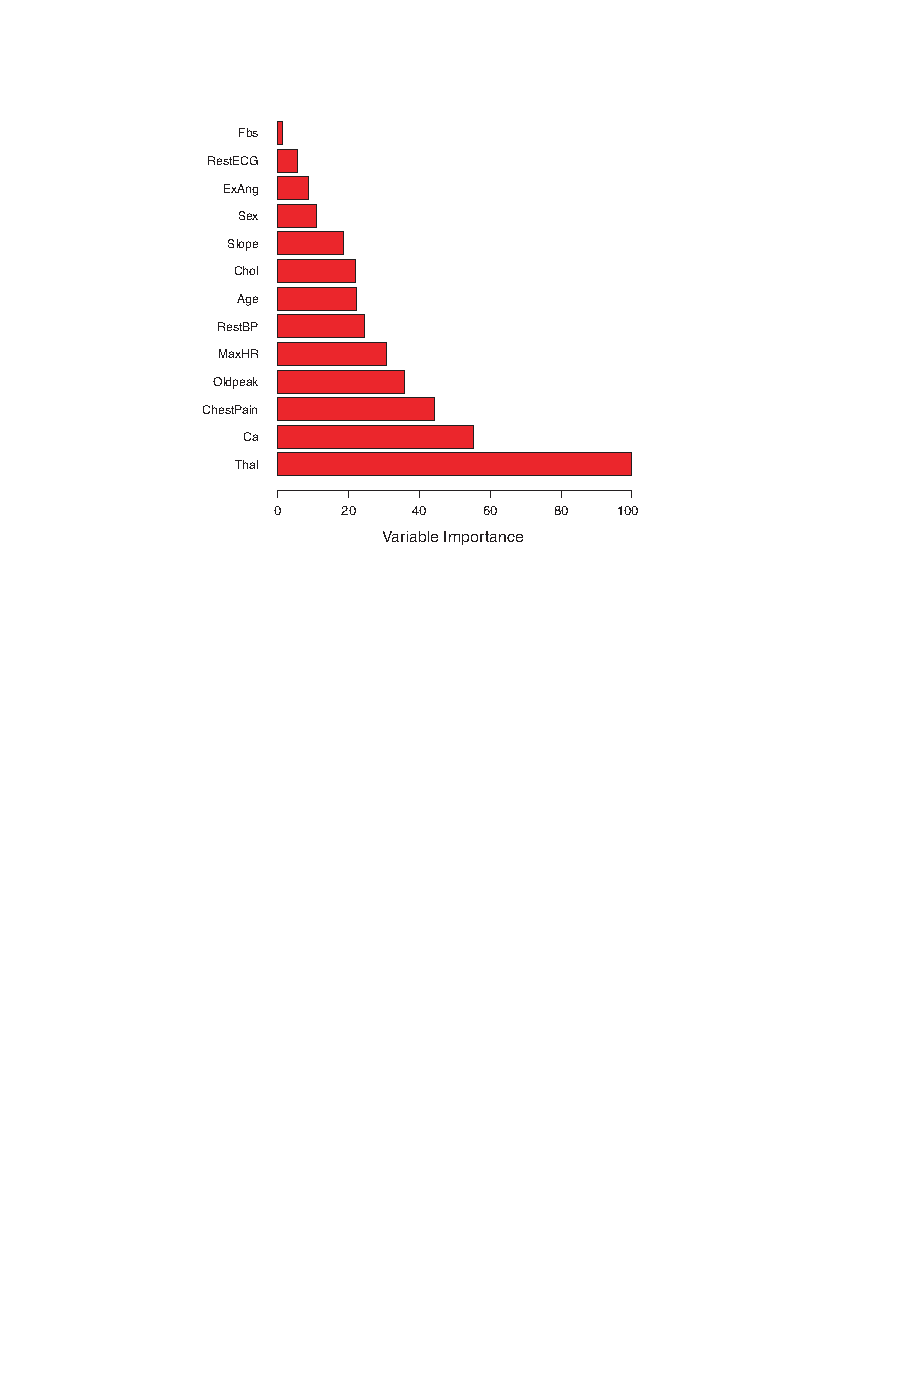
\includegraphics[height=0.8\textheight]{VIM}
\caption*{Thal = Thalium stress test}
\end{figure}
\end{frame}

\begin{frame}{}

\LARGE
\begin{center}
Random Forests (also due to Leo Breiman)
\end{center}
\end{frame}

\begin{frame}{Random Forests are a simple modification to bagging:}

On each split, evaluate only $m<p$ randomly chosen predictors.  \\~\\

Why?  What might this accomplish?\\~\\
\pause

Suppose there is a predictor that is \textit{always} the best first split.  If you always split on it first, the space of subtrees you can grow is limited.  Splitting on only a subset ensures you don't always split on the winner.  
\begin{itemize}
\item This ``decorrelates'' the trees
\item The average has less variance as a result.\\~\\
\end{itemize}
\pause
$m=\sqrt{p}$ works well for classifiers, $m=\frac{p}{3}$ is good for regression.
\end{frame}

\begin{frame}{Let's look at the heart data again}

\begin{figure}
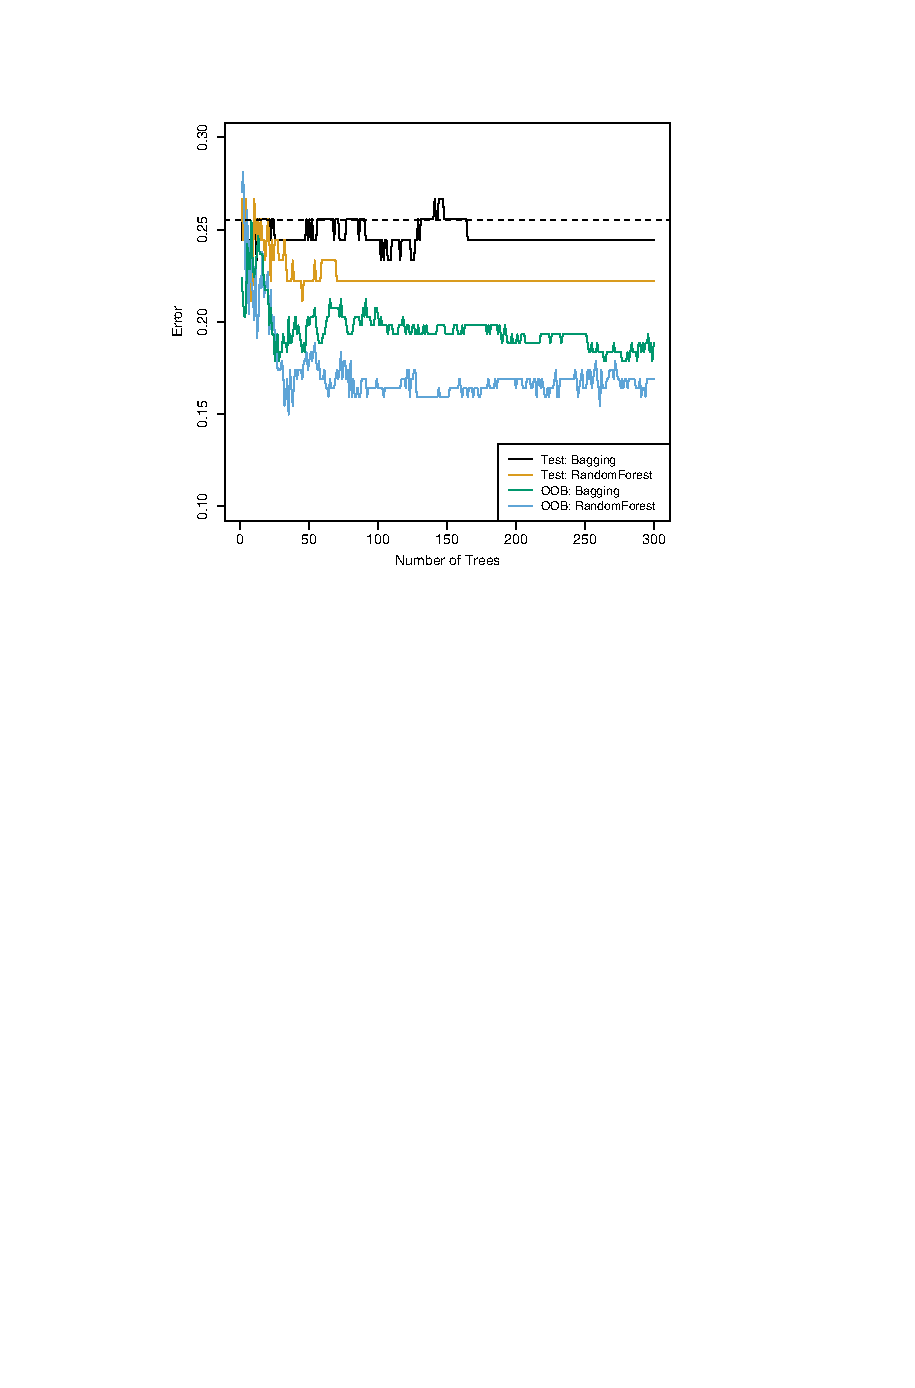
\includegraphics[height=0.85\textheight]{islr88.pdf}
\caption*{}
\end{figure}
\end{frame}

\begin{frame}{}
Let's take the quiz
\end{frame}

\begin{frame}{}
\LARGE
\begin{center}
Boosting
\end{center}
\end{frame}

\begin{frame}{The Boosting algorithm}
\begin{enumerate}
\item Set $\hat{f}=0$ and $r_i =y_i$ for all \textit{i} in the training set.
\item For $b=1,2,...,B,$ repeat:
\begin{enumerate}
\item Fit a tree $\hat{f}_b$ with $d$ splits ($d+1$ terminal nodes) to the training data $(X,r)$.
\item Update $\hat{f}$ by adding in a shrunken version of the new tree:
\begin{align*}
\hat{f}(x) \leftarrow\hat{f}(x)+\lambda \hat{f}^b(x)
\end{align*}
\item Update the residuals
\begin{align*}
r_i \leftarrow r_i - \lambda\hat{f}^b(x_i)
\end{align*}
\end{enumerate}
\item Output the boosted model
\begin{align*}
\hat{f}(x) =\sum_{b=1}^B \lambda \hat{f}^b(x)
\end{align*}
\end{enumerate}
\end{frame}

\begin{frame}{Why does boosting work?}
\pause
It's chasing the residuals for the model.\\~\\
\begin{itemize}
\item instead of choosing new models that explain the data well...
\item ...it chooses models that explain the \textit{residuals} between observations and the ``current'' model\\~\\
\end{itemize}
\end{frame}

\begin{frame}{Comments on boosting}
Tuning parameters:
\begin{enumerate}
\item $B$ is the number of ``boosts''.  Because we're not averaging models fit to the same thing, there is a risk of over-fit.  Choose $B$ via cross validation.
\item $\lambda$ is like the ``learning rate'', and we choose pretty small values (0.001 or 0.01).   This slows down learning and avoids making residuals worse in some places in order to push residuals down on average. 
\item $d$ is the number of splits in each tree.  This can be very low (1 or 2)
\end{enumerate}
\end{frame}

\begin{frame}{}
\begin{figure}
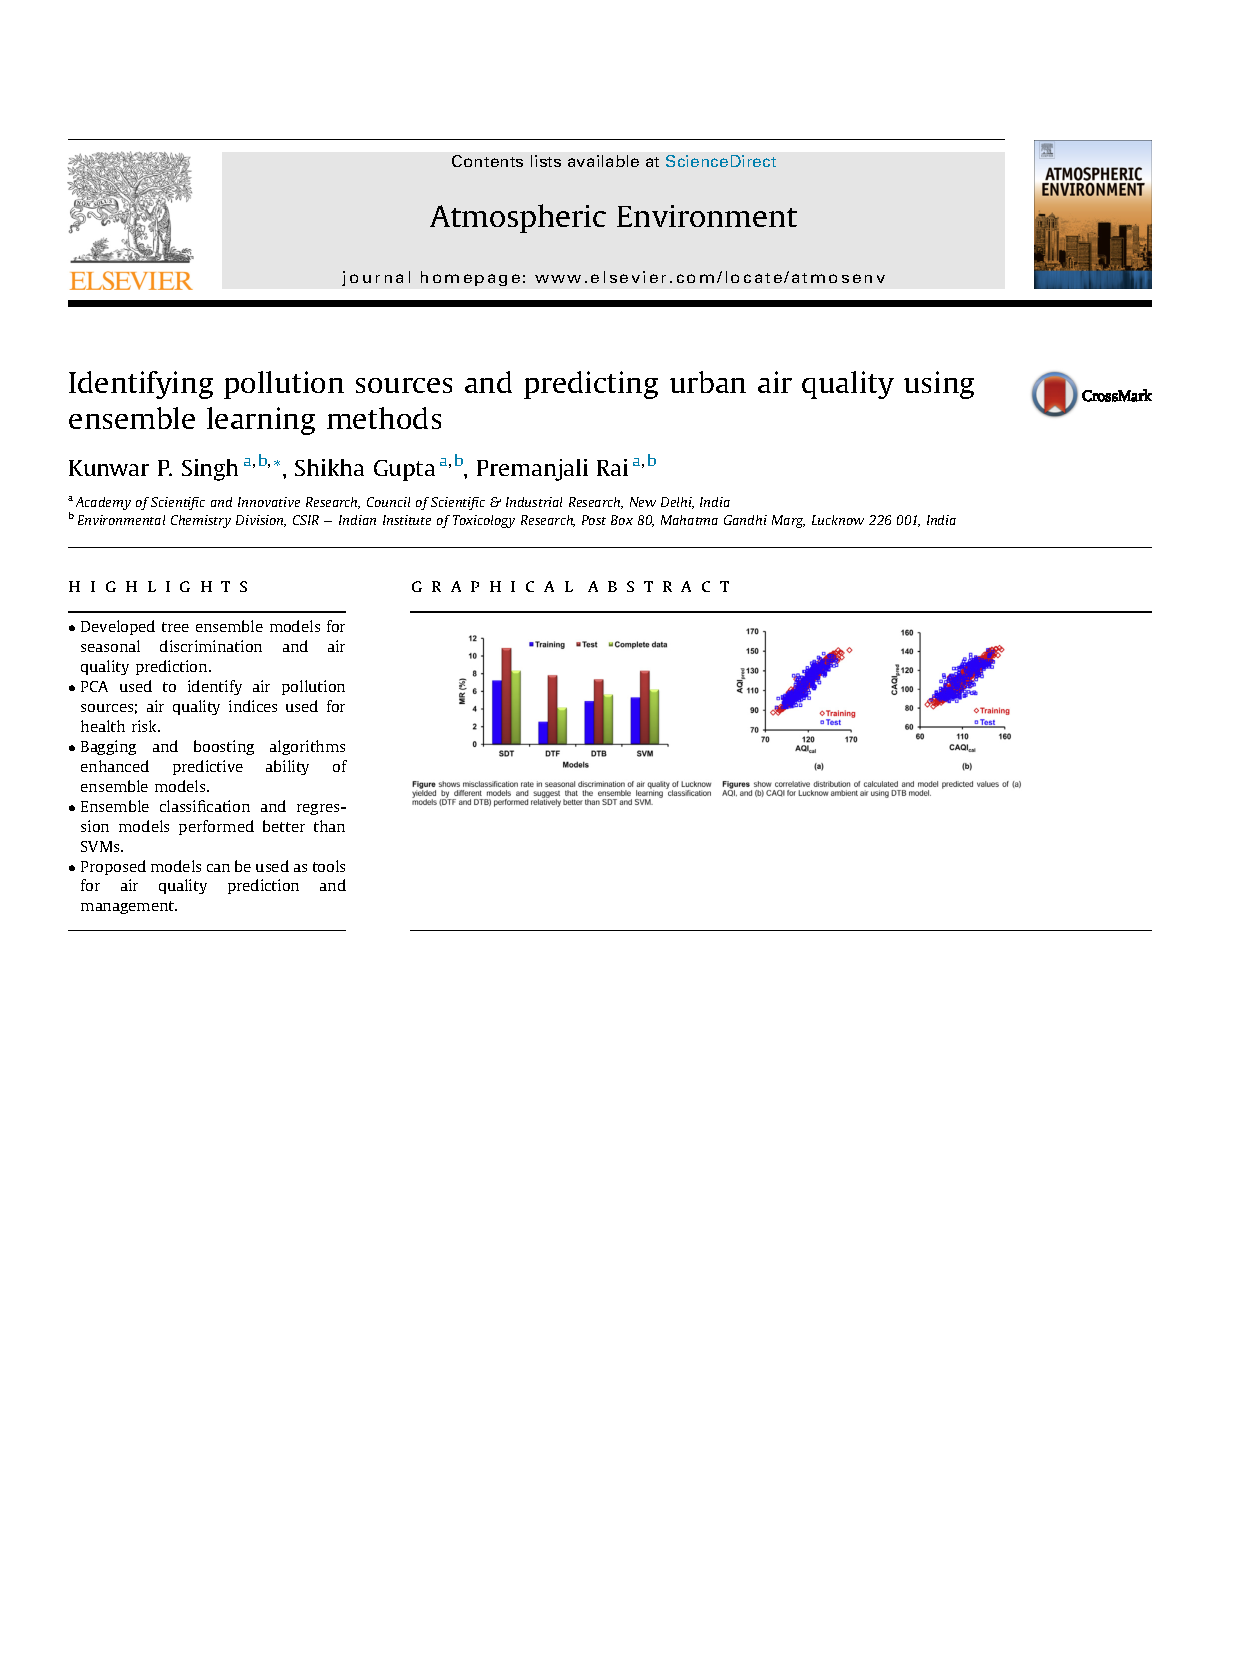
\includegraphics[height=\textheight]{singh_etal}
\caption*{}
\end{figure}
\end{frame}

\begin{frame}{Singh \textit{et al} study region -- Lucknow}
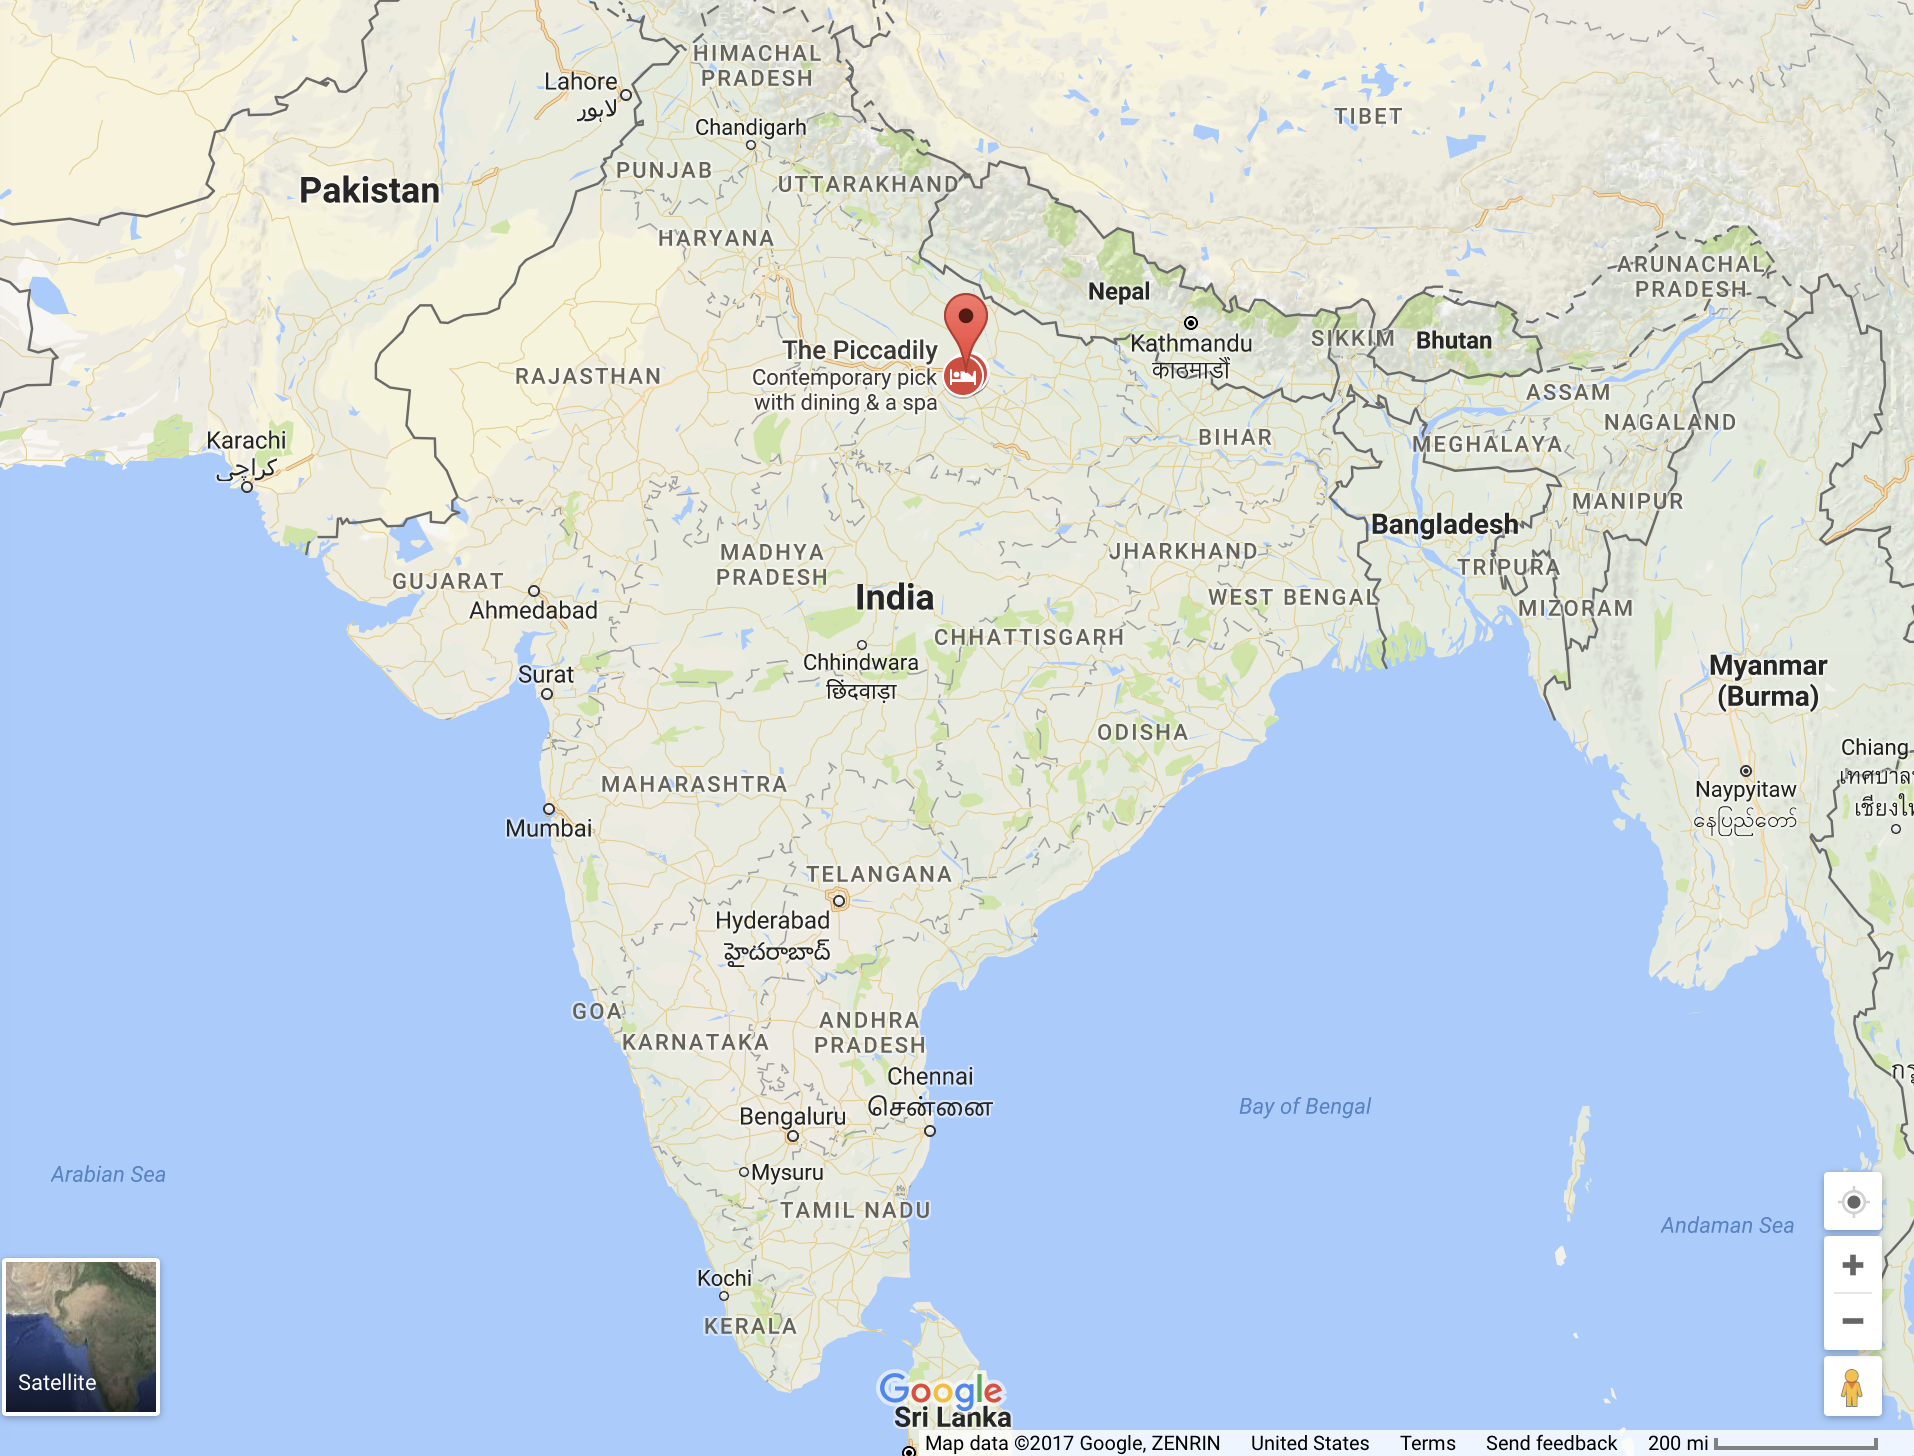
\includegraphics[height=0.9\textheight]{lucknow}
\end{frame}

\begin{frame}{}
\begin{figure}
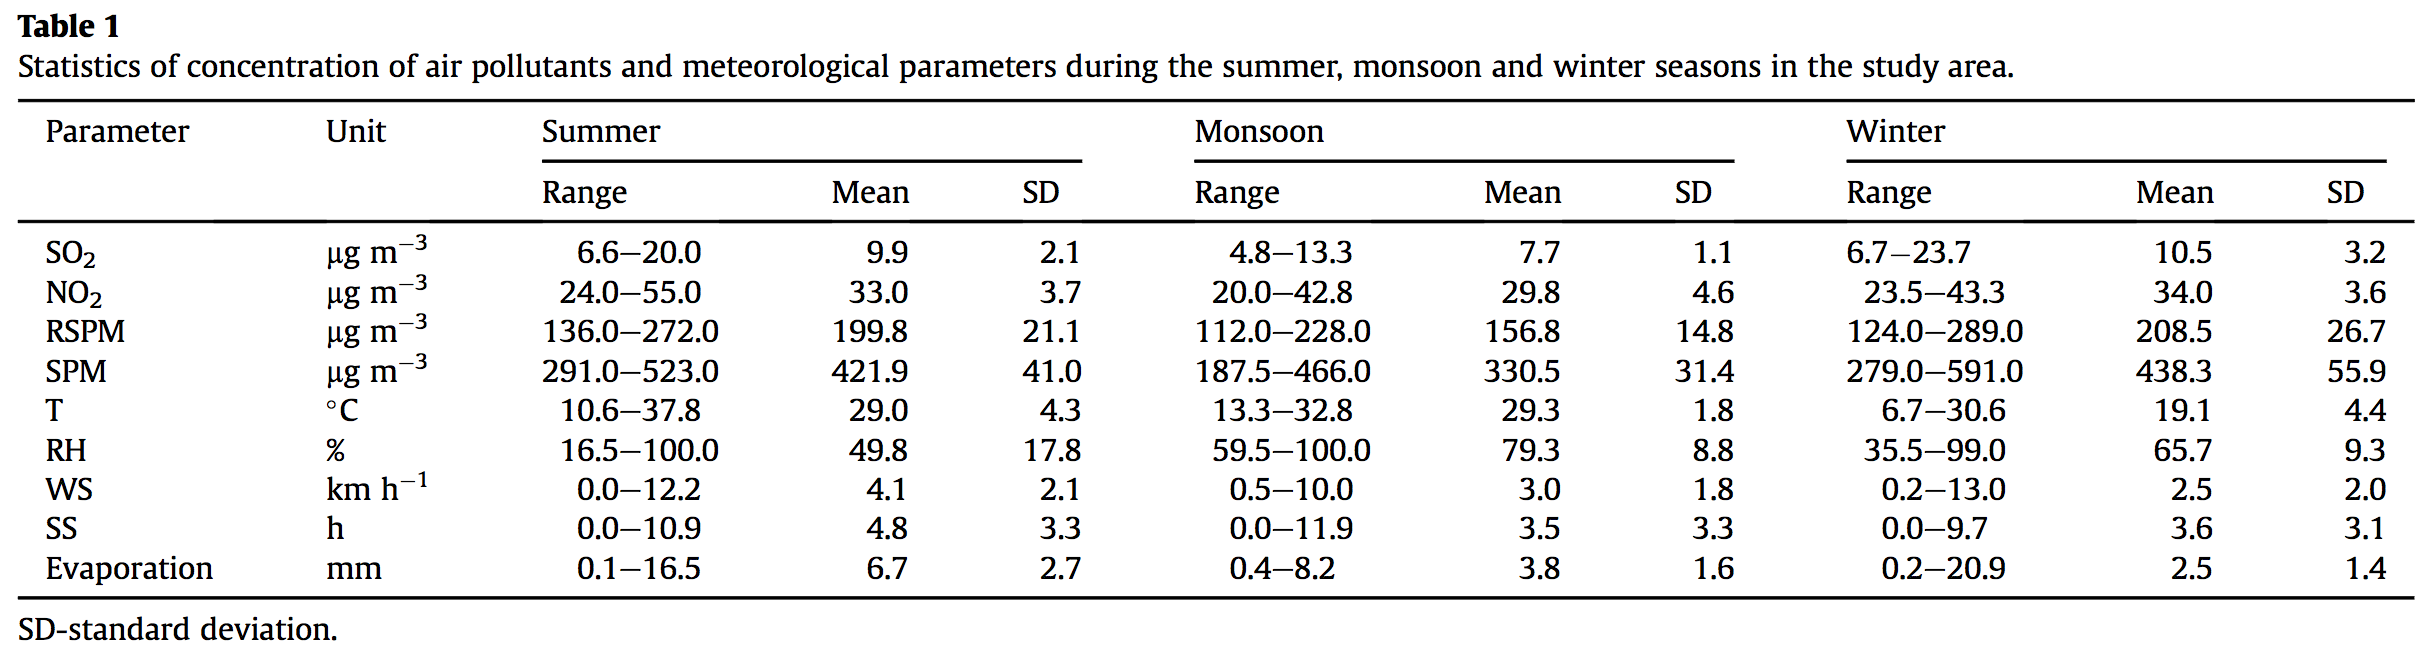
\includegraphics[width=\textwidth]{singh_table1}
\caption*{RSPM = respirable suspended PM10; SPM = suspended PM.  RSPM permissible levels in India = 100 $\mu$g/m$^{-3}$; In U.S., 150 $\mu$g/m$^{-3}$ is unhealthy for sens. groups.}
\end{figure}
\end{frame}

\begin{frame}{Singh \textit{et al} objective and result}

Use ensemble-learning tree-based methods to predict combined AQI using meteorological variables (temp, RH, wind speed, evaporation rate, sun hours)
\begin{columns}
\column{0.75\textwidth}

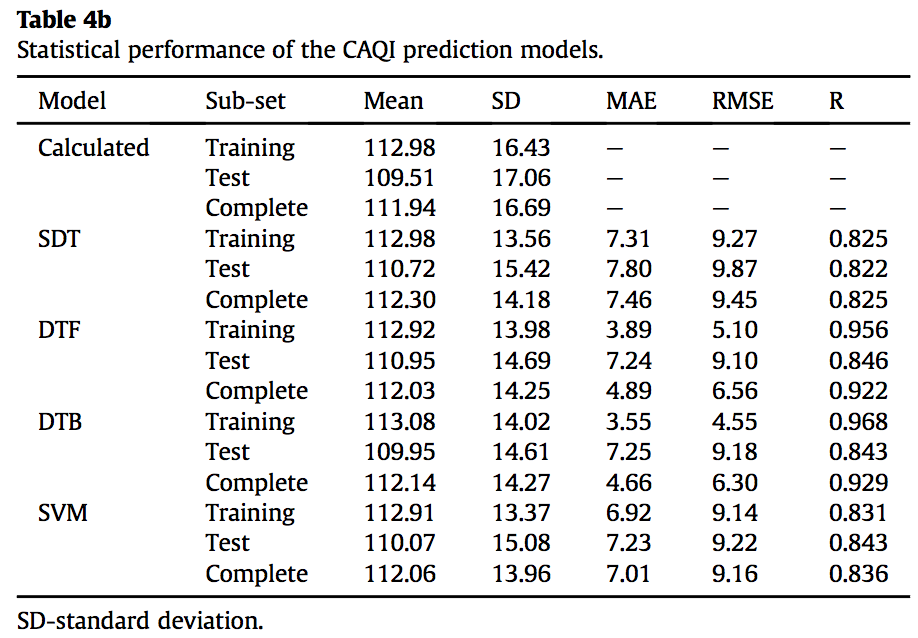
\includegraphics[height=0.75\textheight]{singh_4b}
 

\column{0.25\textwidth}
\footnotesize SDT = single decision tree\\~\\
DTF = decision tree forest\\~\\
DTB = decision tree boosted\\~\\
SVM = support vector machine
\end{columns}
\end{frame}
\end{document}
